% This is samplepaper.tex, a sample chapter demonstrating the
% LLNCS macro package for Springer Computer Science proceedings;
% Version 2.20 of 2017/10/04
%
\documentclass[runningheads]{llncs}
%
\usepackage{graphicx}
% Used for displaying a sample figure. If possible, figure files should
% be included in EPS format.
%
% If you use the hyperref package, please uncomment the following line
% to display URLs in blue roman font according to Springer's eBook style:
% \renewcommand\UrlFont{\color{blue}\rmfamily}

\begin{document}
%
\title{Video Player Architecture for Virtual Reality on Mobile Devices\thanks{Supported by Sidia}}
%
%\titlerunning{Abbreviated paper title}
% If the paper title is too long for the running head, you can set
% an abbreviated paper title here
%
\author{Adriano M. Gil \and
Afonso R. Costa Jr \and
Atacilio C. Cunha \and
Thiago S. Figueira \and
Antonio A. Silva}


%
\authorrunning{F. Author et al.}
% First names are abbreviated in the running head.
% If there are more than two authors, 'et al.' is used.
%
\institute{SIDIA Instituto de Ci\^encia e Tecnologia (SIDIA)\\
Manaus, Brazil
\email{\{adriano.gil,afonso.costa,atacilio.cunha,\\
         thiago.figueira,antonio.arquelau\}@sidia.com}}
%
\maketitle              % typeset the header of the contribution
%
\begin{abstract}
% TODO: write abstract
The abstract should briefly summarize the contents of the paper in
150--250 words.

\keywords{virtual reality  \and mobile \and video player \and architecture}
\end{abstract}
%
%
%
\section{Introduction}
 % Afonso

Virtual Reality (VR) applications provide great interaction with multimedia content. This kind of content becomes an unique experience for the end-user as applications work as a media gallery inside the VR environment such as the Samsung VR \cite{SVR}.

Those applications, which are usually built using 3D engines or frameworks, target mobile devices like smartphones. There are two 3D engines used for creating such applications for mobile devices (mainly for Android platform): Unity \cite{Unity} and Samsung XR (SXR) \cite{SXR}. Those engines are good choice but it is important to mention that the applications will be run in a mobile platform, which has limited resources like memory, battery and computational power. In this scenario, it is important to define and follow a software architecture to organize the communication between the render and platform layers, thus provide better performance results.

Mobile platforms like Android has already its native media player. This kind of application has its architecture and components well defined and designed to take advantages regarding performance and resource consumption. It means that the media codecs were chosen/defined and are organized to support the most common media formats and data sources. Therefore, a video player application is built using two main parts: a media player (that takes digital media in and renders it as video) and a media controller (generally an User Interface - UI, with transport controls to run the player and optionally display the player's state).

Video player applications that are being built for VR environments need to have this kind of organization as well, once they are using 3D engines to render digital media.

This work proposes a high-performance architecture that can be implemented for video players on mobile platforms to run videos on VR environments. This architecture is evaluated using two 3D engines: Unity and SXR in the Android platform.

The structure of this paper is as follows. In section \ref{related-work}, we provide an overview of the video players usage in VR context. Then, in section 3, the methodology used in this work will be detailed. In section \ref{architecture}, the proposed architecture will be shown and explained. Finally in section \ref{conclusion}, we will provide some concluding remarks.


\section{Related Work} \label{related-work}

% Gil

Media consumption is a relevant activity for users in the digital world, and it has been growing according to \cite{repo2004users}. In this work this consumption is shown as a way to deal with tedious situations, sharing experience and sharing knowledge.

Applications can use the media consume as a way to create an specific interactions with the user. In \cite{hu2018kalgan}, is cited an example of applications to language learning using a video player focusing on language manipulation inside the media.

In \cite{smolic2009overview}, are listed different codecs that can by used o stereoscopic videos transmission, where reinforces the idea that depth component can by compressed in any ways.

The work \cite{wild2018inaccessibility} mentions the need to adapt Video Players to being accessible to people with special needs. According to the article it is necessary that the Video Player has subtitles support, audio description, media transcriptions, support for change volume and color contrast.

MR360 defined in \cite{rhee2017mr360} proposes a composition of 3D virtual objects during a 360 video execution. The panoramic video is used both as a light source to illuminate virtual objects how much to compose the backdrop to be rendered.

% TODO: Refs regarding Sw architectures for VR apps
% TODO: Current solutions for developping media players on VR

\section{Methodology} \label{methodology}

The following methodology is being used to to evaluate the proposed architecture:

\begin{enumerate}
    \item Definition of the video format.
    \item Definition of ways to visualize the video in a virtual environment.
    \item Comparison between two different render implementations (Unity and SXR) in the Android platform (using two different devices).
    \item Comparison between two different native video players (ExoPlayer \cite{Exo} and Android Player \cite{AndroidVideoPlayer}).
\end{enumerate}

The chosen videos are 360-degree videos in the \textit{.mp4} format since this format is widely used in Android devices. The performance evaluation tool is the OVR Metrics Tool \cite{ovrmetrictool}, and the metric is frame-rate (FPS), which is most significant for the user experience.

% TODO: Which metrics we are going to use to compare different architectures? Why?

%In a VR environment, will be made media types manipulation, for example: audio, image and video. With this options, the video media format was chosen for the experiments of this paper. So an architecture that has a good performance at mobile devices will be proposed.

\section{VR Video Player}
% Antonio
% TODO: List features of a VR video player
% TODO: List dependencies necessary to build a VR video player app: media decoder, rendering engine, ...
% TODO: What are the non-functional requirements of such apps?

\section{Architecture} \label{architecture}

% TODO: Describe how such components are connected
% TODO: Describe how non-functional requirements can be met with this architecture

Seeking for an optimized way to use a video player in mobile virtual reality platforms, the architecture was divided into two main layers:

\begin{enumerate}
    \item Platform layer: native implementation to handle I/O operations and file system.
    \item Rendering layer: use of some render framework to turn visible inside the 3D virtual universe.
\end{enumerate}

This architecture (Figure \ref{fig-video-player-arch}) aims to (1) organize the communication between all modules present in the layers, (2) organize the code to be used by different render engines or different native players, and (3) provide good performance in all media codecs and texture renders.

The Platform layer is responsible for media consuming, file system, allocation and memory management. Some multimedia application that executes videos needs not only render digital media but allow user interact with this player.

\begin{figure*}[h!]
    \centerline{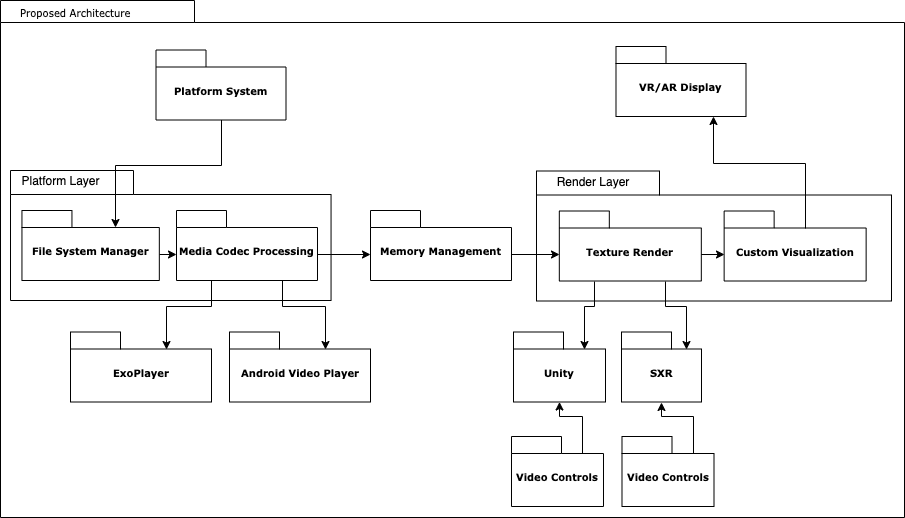
\includegraphics[scale=0.5]{images/ProposedArch.png}}
    \caption{Proposed architecture for Video Player}
    \label{fig-video-player-arch}
\end{figure*}

\subsection{Render layer}
% afonso

\subsection{Platform layer}
% Atacilio
The Platform layer is composed by two parts that provide the baseline for the Video Player Architecture for Virtual Reality on Mobile Devices. They are:

\begin{itemize}
    \item \textit{File System Manager}: in charge of the media file usage and organization;
    \item \textit{Media Codec Processing}: process media files that are loaded for Render Layer.
\end{itemize}

These parts will be clarified in the following sections.

\subsubsection{File System Manager}

The main objective of File System Manager is to provide a centralized and organized data layer composed of multimedia files. This layer must provide all files transparently so that the player has an unique way of working with any type of media.

\begin{figure*}[h!]
    \centerline{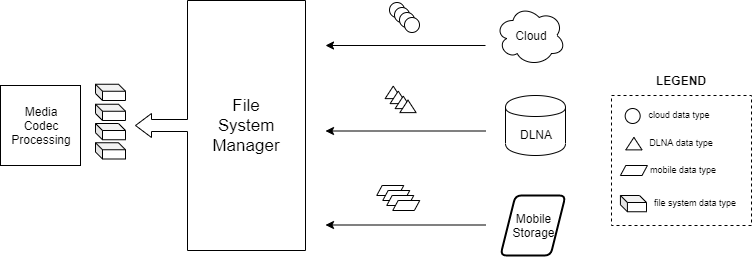
\includegraphics[scale=0.5]{images/file_system2.png}}
    \caption{File System Manager environment}
    \label{fig-file-system}
\end{figure*}

A robust file system manager must implement an interface to output data in order the video player knows how to handle it even though it comes from different types of sources as it's shown on figure \ref{fig-file-system}. In this case,
the file system manager needs to parse all data received from any cloud server, own mobile storage or even a DLNA (\textit{Digital Living Network Alliance}) server and use a defined interface to provide an unique data type that will be processed by Media Codec.

\subsubsection{Media Codec Processing}

Any multimedia application that plays video must not only render digital media,
but it also needs controls to interact with as well as provide status about the currently playing file.
These requirements are important for users, considering they define the possibilities each media player provides.

In the Android platform, it is possible to create a media player using one of the following technologies:

\begin{itemize}
    \item \textit{Media Player class}: provides basic controls to reproduce audio and video files;
    \item \textit{Exo Player library}: the ExoPlayer \cite{ExoPlayer, ExoPlayerHello} library defines standards for audio and video reproduction.
 It was built using the MediaCodec API with features such as DASH
 (\textit{Dynamic Adaptive Streaming over HTTP}) and HLS (\textit{HTTP Live Streaming}), which are not available in the MediaPlayer class.
\end{itemize}

\begin{figure*}[h!]
    \centerline{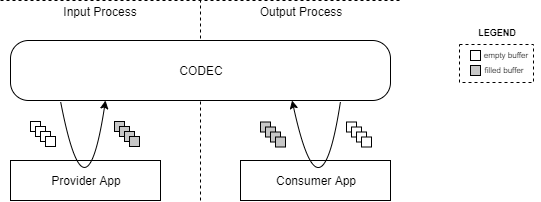
\includegraphics[scale=0.5]{images/codec.png}}
    \caption{Codec process}
    \label{fig-codec}
\end{figure*}

The MediaCodec class offers several possibilities for ExoPlayer by giving access to media codecs at a
low level of implementation. This is possible because codecs convert input data
into output data through multiple I/O buffers processed asynchronously (see figure \ref{fig-codec}).

MediaCodec has the following types of data: compressed, raw audio, raw video. Any of these types can be processed using objects of the ByteBuffer class.

The codec performance is improved when Surface is used for raw video data. This is due to the use of native buffers where it is not necessary to map or copy data for ByteBuffers objects. It is worth mentioning that it is impossible to access raw data when using a Surface. In this case, an object of the ImageReader class is necessary to obtain video frames.

The mimetype of a file defines the compressed data for the input and output buffers. For videos, it is usually just a single frame of compressed video. Regarding video buffers in ByteBuffer mode, they are defined according to the color format that can be \textit{native raw video format}, \textit{flexible YUV buffers} or \textit{others} - generally supported by the ByteBuffer mode through specific format.

As presented on \cite{MediaCodec}, every codec has states that map actions during its life cycle. They can assume the \textit{Stopped}, \textit{Executing} and \textit{Released} states. The Stopped state maps a set of other sub-states that are \textit{Uninitialized}, \textit{Configured} and \textit{Error}. The Executing state builds on other sub-states that are \texit{Flushed}, \textit{Running} and \texit{End-of-Stream}.

One of the most important points related to performance in multimedia applications is the use of \textit{OpenGL for Embedded Systems (OpenGL ES)} API. OpenGL is a programming interface that allows communication and manipulation of 3D graphics processing on hardware. Android supports the OpenGL ES versions 1.0 and 1.1 (Android 1.0+), 2.0 (Android 2.2+), 3.0 (Android 4.3+)\footnote{Perhaps a device running Android 4.3+ does not support OpenGL ES 3.0. To check which version of the OpenGL ES API is supported, you need to specify the minimum version of OpenGL ES in the application's manifest or check through OpenGL ES context which version is available.} and 3.1 (Android 5.0).

Rendering in textures is not so discussed and is one of the least documented parts of literature. The use of textures allows the updating and continuous rendering of dynamic components such as websites, videos and others. For static objects, the best approach is to work with bitmap. The manipulation of graphics through the OpenGL ES API takes place from the GLSurfaceView class and the GLSurfaceView.Renderer interface.

The GLSurfaceView class is a View used to draw and manipulate objects through calls made to the OpenGL ES API. The GLSurfaceView.Renderer interface is responsible for making OpenGL calls to render a frame by specifying the following methods that need to be implemented:

\begin{itemize}
    \item \textit{onSurfaceCreated()}: usually called once to define the OpenGL environment parameters that will be used during execution or to initialize API objects;
    \item \textit{onDrawFrame()}: called each time the GLSurfaceView needs to be redrawn;
    \item \textit{onSurfaceChanged()}: called whenever the geometry of the GLSurfaceView is changed, including GLSurfaceView size settings and device screen orientation.
\end{itemize}

In this context, it is known that applications that use the OpenGL ES API commonly create several textures during its execution time. In this case, the higher the resolution textures, the better the graphics are. But with the increased resolution,  more memory is required for management, and more time is spent during texture loading. One way to improve the application's performance, battery consumption, device heating and even decrease the size of the generated APKs is to make use of hardware accelerated formats.

The main point of defining textures that are created for video rendering is their definition as \textit{GL\_TEXTURE\_EXTERNAL\_OES} instead of \textit{GL\_TEXTURE\_2D}. This is because OES textures have a semi-global texture table on the GPU that allows them to be used in other GL contexts, thus ensuring safety in their use.

\subsection{Experiments and Results} \label{experiments}
% Antonio
The experiments were made using three different applications: VR Gallery, SXR Video player, and a demo app. The first application is a fully-featured Unity application supporting many other parallel features besides video player; the second one is a video player application on the SXR platform, and the last one is a dump Unity application that implements the architecture presented in this paper.

The graphs below shows the FPS registered in the VR Gallery application.

\begin{figure}[h]
    \centering
    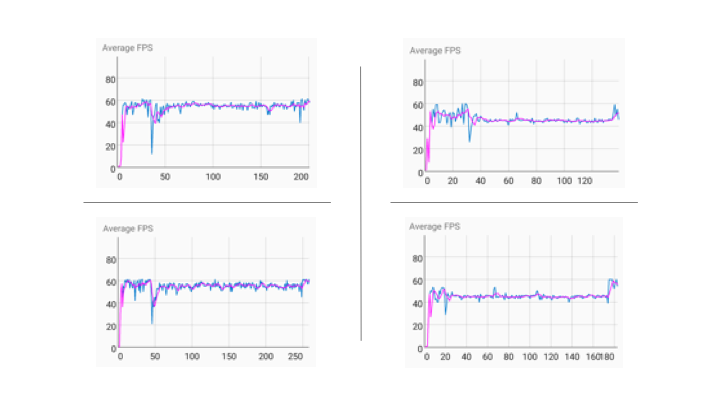
\includegraphics[width=\textwidth]{images/Gallery.png}
    \caption{FPS in VR Gallery}
    \label{gallery-graph}
\end{figure}

According to figure \ref{SXR-graph} and figure \ref{gallery-graph}, the SXR framework maintains 60 FPS in all test cases. However, the initial experiments have shown that the video player of the VR Gallery (application developed in Unity) does not perform well. While in Samsung Galaxy S8 Gallery has a variation between 55 and 60 FPS, in Samsung Galaxy S6 it stays between 40 and 50 FPS. The reason for these results is the heavy environment VR Gallery has, which is not seen in the other applications.

Even with the mentioned remarks, the user experience was not affected in any of the tests as the video player performed well. The user cannot perceive the difference between both applications and the frame-rate difference is unnoticeable.

The graph below shows the FPS registered by SXR application:

\begin{figure}[h]
    \centering
    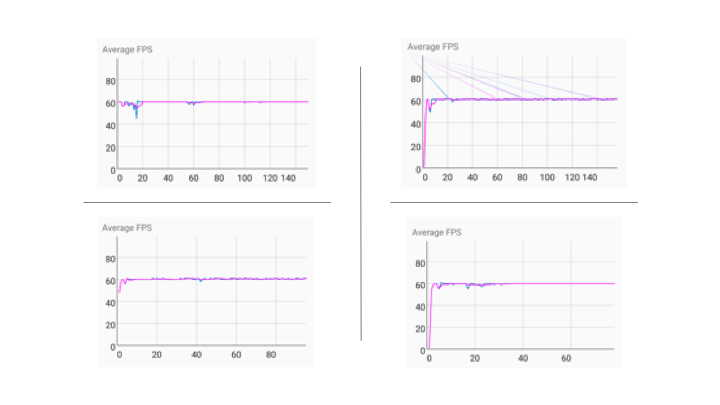
\includegraphics[width=\textwidth]{images/SXR.png}
    \caption{FPS on SXR}
    \label{SXR-graph}
\end{figure}

The difference between both applications is visible. The SXR application has better results, considering its FPS count is around 60 with some small variations. Even though this is a good result, a better behavior can be observed in the last application where the FPS only varies during the application loading and is stable during video execution.

\begin{figure}[!h]
    \centering
    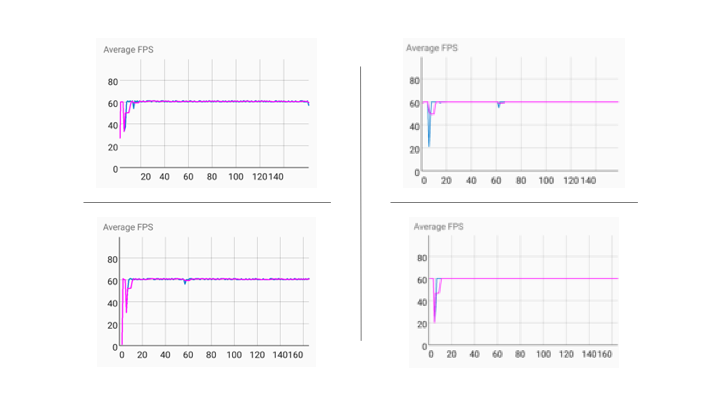
\includegraphics[width=\linewidth]{images/SeparetedApp.png}
    \caption{FPS in the isolated application.}
    \label{app-graph}
\end{figure}


\subsection{Conclusion / Next Steps} \label{conclusion}
% Antonio
% TODO: Highlight main contributions of the paper\
According to the tests, the VR Gallery video player does not have good performance when compared to SXR, however the difference between the two can be explained by the fact that the VR Gallery is a complete and robust application, i.e. it has providers and animations. Even so, the video player of Gallery gives users a complete experience of a good performance video player in a VR environment.

% TODO: Describe next steps
For the full paper, other tests will be made using this architecture in Unity, but isolating the video player from any application. The same metrics will be used but the comparisons will be more directed to the architecture. Besides that, different native video players will be tested using the architecture as well.

%
% ---- Bibliography ----
%
% BibTeX users should specify bibliography style 'splncs04'.
% References will then be sorted and formatted in the correct style.
%
\bibliographystyle{splncs04}
\bibliography{vrvideoplayerarch}

\end{document}
